\documentclass[12pt]{article}
%\usepackage{tkiz}

\usepackage[utf8]{inputenc}
\usepackage[french]{babel}
\usepackage{amsmath,amsthm,amsfonts,amssymb}
\usepackage{lmodern}
\usepackage[top=2.4cm,bottom=2.4cm,left=2cm,right=2cm]{geometry}
\usepackage{hyperref}
\usepackage{multicol}
\usepackage{enumitem}
\usepackage{listings}
\usepackage[dvipsnames]{xcolor}
\usepackage{tikz}
\author{MABROUK Fayez}
%\date{}
\title{{\bf  Génie Logiciel} \\
	Compte rendu TD08  \\
	{\small L3 Informatique appliquée 2022-2023} \\
	{\it \small \no étudiant : 22213839 }}
\begin{document}
	\maketitle
	\newpage
	\section{Diagramme de séquence}
	Pour chacun des cas d’utilisations du système bibliothèque développés la semaine dernière,
	proposez un diagramme de séquence.
	\begin{figure}[!hbtp]
		\centering
		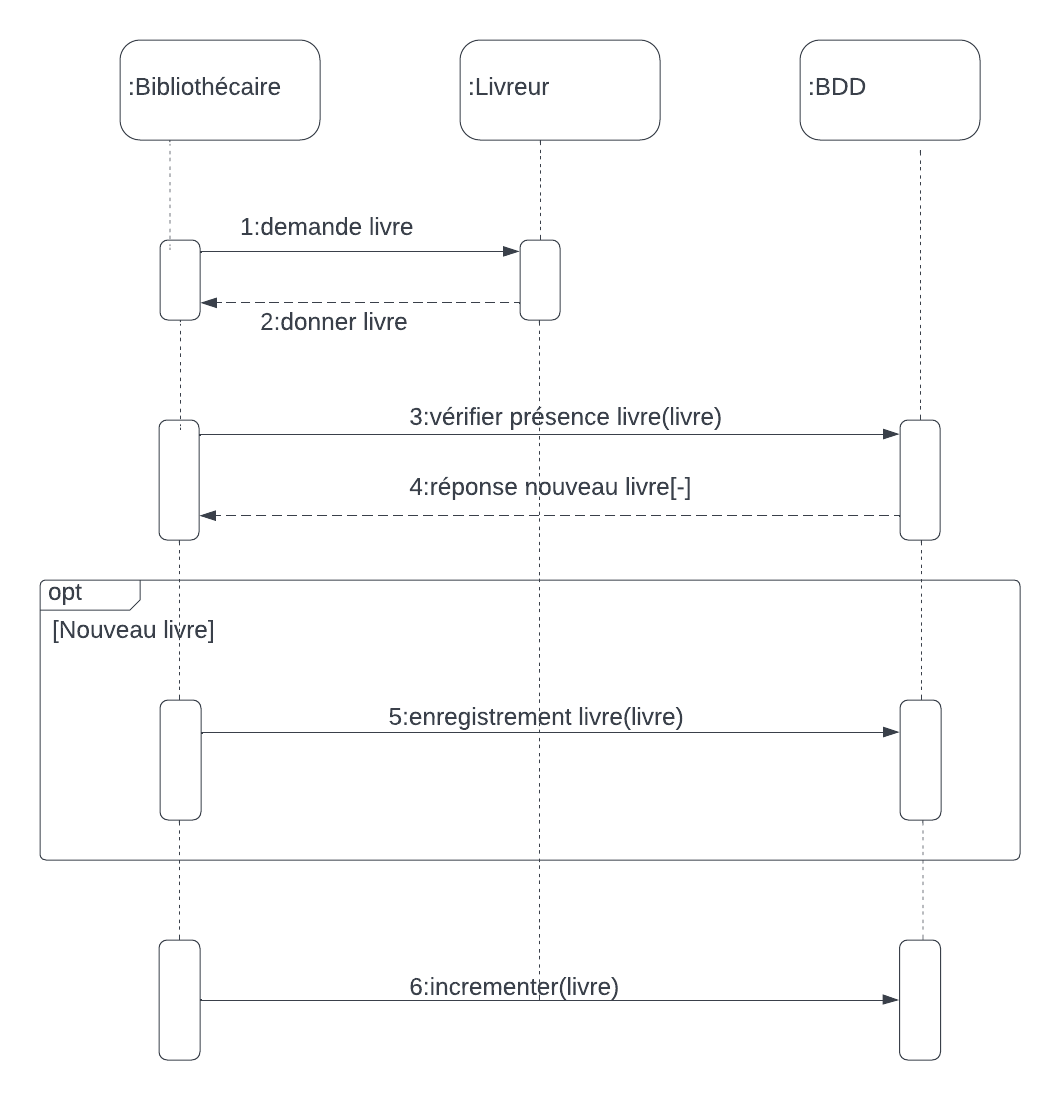
\includegraphics[scale=0.75]{capture1_S.png}
		\caption{Diagramme de séquence 1}
	\end{figure}
\newpage
\begin{figure}[!hbtp]
	\centering
	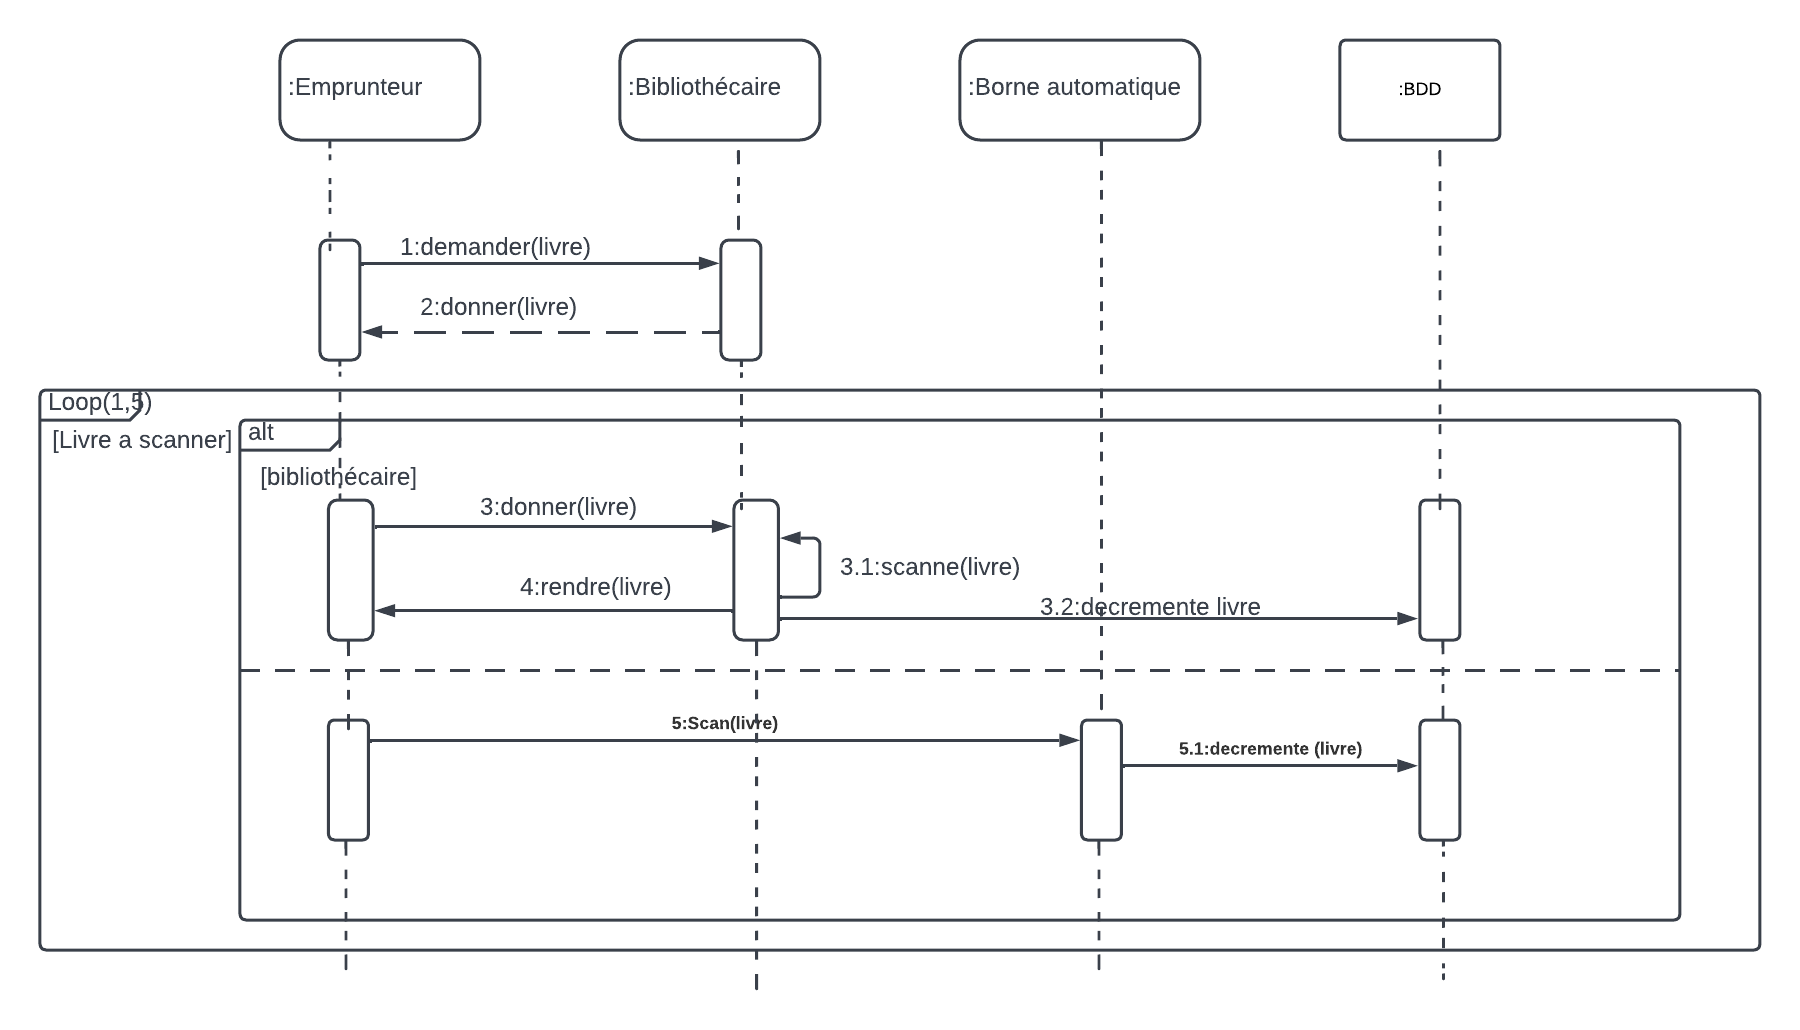
\includegraphics[scale=0.65]{capture2_S.png}
	\caption{Diagramme de séquence 2}
\end{figure}
	\end{document}